Consider the supply and demand curve for a product. Recall that the supply curve is always increasing and the demand curve decreasing.

\begin{image}
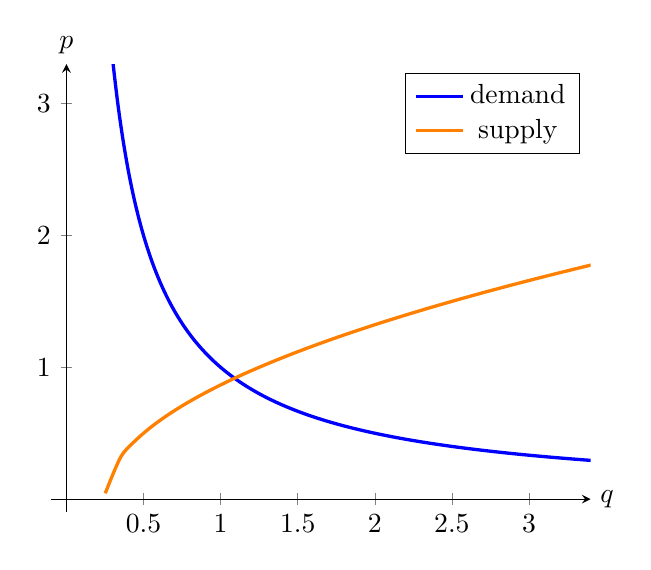
\begin{tikzpicture}
  \begin{axis}[
  xmin=-0.1,
  xmax=3.4,
  ymin=-.1,
  ymax=3.3,
  axis lines=center,
  xlabel=$q$,
  ylabel=$p$,
  every axis y label/.style=
    {at=(current axis.above origin),anchor=south},
  every axis x label/.style=
    {at=(current axis.right of origin),anchor=west},
  ]
\addplot [very thick, blue, smooth, samples=100, domain=0.1:3.4] {1/x};
\addlegendentry{demand}
\addplot [very thick, orange, smooth, samples=100] {(x-0.25)^0.5};
\addlegendentry{supply}
\end{axis}
\end{tikzpicture}
\end{image}

Suppose we set the initial price at \(1.5.\) Then how does the supply and demand quantity associated with that price compare?

\begin{image}
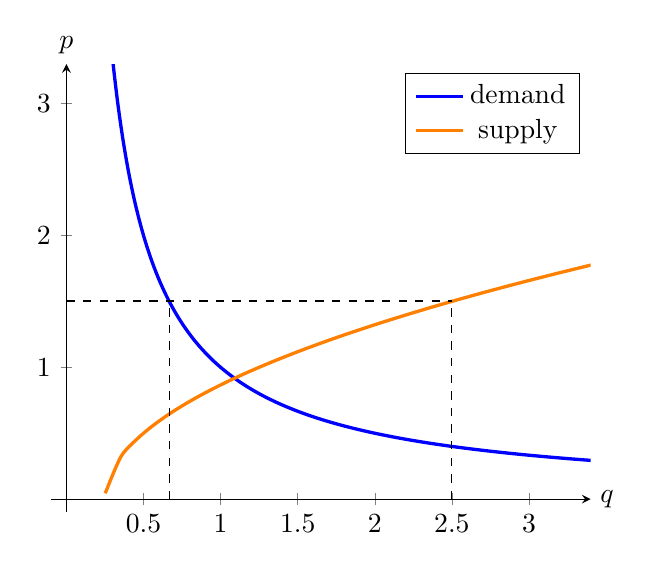
\begin{tikzpicture}
  \begin{axis}[
  xmin=-0.1,
  xmax=3.4,
  ymin=-.1,
  ymax=3.3,
  axis lines=center,
  xlabel=$q$,
  ylabel=$p$,
  every axis y label/.style=
    {at=(current axis.above origin),anchor=south},
  every axis x label/.style=
    {at=(current axis.right of origin),anchor=west},
  ]
\addplot [very thick, blue, smooth, samples=100, domain=0.1:3.4] {1/x};
\addlegendentry{demand}
\addplot [very thick, orange, smooth, samples=100] {(x-0.25)^0.5};
\addlegendentry{supply}
\addplot[dashed, thick, domain=0:2.5]{1.5};
\addplot[dashed] coordinates {(2.5,0) (2.5,1.5)};
\addplot[dashed] coordinates {(0.67,0) (0.67,1.5)};
\end{axis}
\end{tikzpicture}
\end{image}

From the graph we can see that there is \emph{demand} for less than what can be supplied at this price. That is, there is a \emph{surplus.} From the demand curve, we see that in order to sell a supply of \(2.5,\) we would need to set the price at around \(0.4.\) But at this price, the amount we can sell is greater than the supply. There is a \emph{shortage.}

\begin{image}
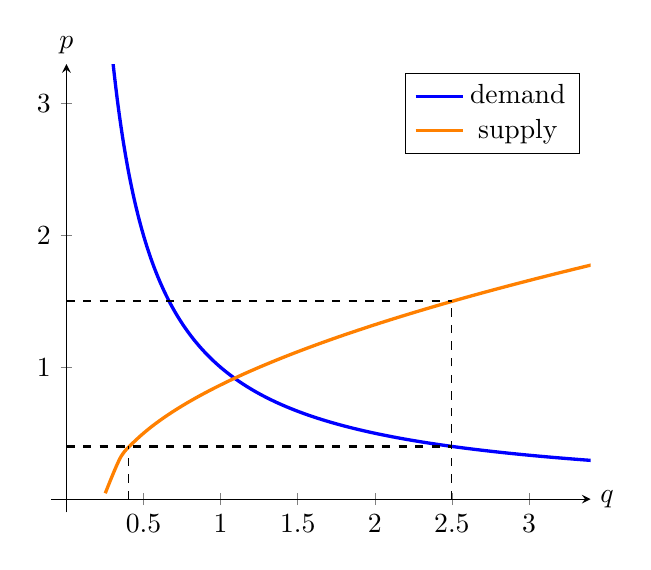
\begin{tikzpicture}
  \begin{axis}[
  xmin=-0.1,
  xmax=3.4,
  ymin=-.1,
  ymax=3.3,
  axis lines=center,
  xlabel=$q$,
  ylabel=$p$,
  every axis y label/.style=
    {at=(current axis.above origin),anchor=south},
  every axis x label/.style=
    {at=(current axis.right of origin),anchor=west},
  ]
\addplot [very thick, blue, smooth, samples=100, , domain=0.1:3.4] {1/x};
\addlegendentry{demand}
\addplot [very thick, orange, smooth, samples=100] {(x-0.25)^0.5};
\addlegendentry{supply}
\addplot[dashed, thick, domain=0:2.5]{1.5};
\addplot[dashed, thick, domain=0:2.5]{0.4};
\addplot[dashed] coordinates {(2.5,0) (2.5,1.5)};
 \addplot[dashed] coordinates {(0.4,0) (0.4,0.4)};
\end{axis}
\end{tikzpicture}
\end{image}

Since there is a surplus at \(1.5\) and a shortage at \(0.4\), we operate under the assumption that this means there is a price between \(1.5\) and \(0.4\) such that \(demand = supply.\) This is called the point of equilibrium for a product. We can hopefully approximate this point of equilibrium by taking the average of the two prices. In our case, \((1.5+0.4)/2 = 0.95.\) From the graph of our function it appears that \(0.95\) is around the equilibrium price.

\begin{image}
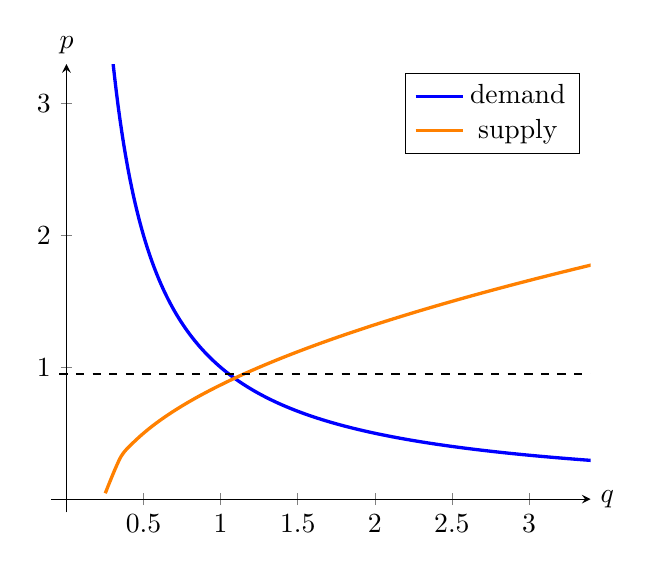
\begin{tikzpicture}
  \begin{axis}[
  xmin=-0.1,
  xmax=3.4,
  ymin=-.1,
  ymax=3.3,
  axis lines=center,
  xlabel=$q$,
  ylabel=$p$,
  every axis y label/.style=
    {at=(current axis.above origin),anchor=south},
  every axis x label/.style=
    {at=(current axis.right of origin),anchor=west},
  ]
\addplot [very thick, blue, smooth, samples=100, domain=0.1:3.4] {1/x};
\addlegendentry{demand}
\addplot [very thick, orange, smooth, samples=100] {(x-0.25)^0.5};
\addlegendentry{supply}
\addplot[dashed, thick]{0.95};
\end{axis}
\end{tikzpicture}
\end{image}

\begin{definition}
    The \emph{point of equilibrium} for a product is the oint of intersection for the supply and demand curves. If this point is \(\left(m,n\right)\) then the price \(n\) is the \emph{equilibrium price}, the quantity \(m\) is the \emph{equilibrium quantity}.
\end{definition}

The supply and demand curves form system of two equations in the variables \(p\) and \(q!\) Finding the equilibrium point amounts to solving the system of equations.